\documentclass[10pt, aspectratio=169]{beamer}

\usefonttheme{serif}
\usepackage[T1]{fontenc}

\title[Séminaire LVMT]{Agrégation d'enquêtes mobilité pour analyser l'intermodalité : enseignements tirés de 78 enquêtes françaises}
\date[24 novembre 2025]{Séminaire LVMT\\24 novembre 2025}
\author{Lucas Javaudin}
% \institute[]{THEMA, CY Cergy Paris Université}

% \usepackage{pgfpages}
\usepackage{siunitx}
\usepackage{booktabs}
\usepackage{graphicx}
\usepackage{amssymb}
\usepackage{eurosym}
\usepackage{soul}

\sisetup{per-mode=symbol}

\usepackage{tikz}

\usetikzlibrary{shapes.geometric, arrows.meta, positioning}

\tikzstyle{startstop} = [rectangle, draw=black, fill=gray!20, rounded corners=5pt, text centered, minimum height=1cm]
\tikzstyle{process} = [rectangle, draw=black, fill=orange!10, minimum height=1.2cm, text centered, rounded corners]
\tikzstyle{io} = [trapezium, trapezium left angle=70, trapezium right angle=110, trapezium stretches=true, draw=black, fill=blue!10, text centered, minimum height=1.2cm]
\tikzstyle{decision} = [diamond, draw=black, fill=yellow!20, aspect=2, text centered, minimum width=1.5cm, minimum height=1cm, inner sep=0pt]
\tikzstyle{arrow} = [thick, ->, >=stealth]

\DeclareSIUnit{\euro}{\text{\euro}}
% \sisetup{per-mode=single-symbol}

\newcommand{\red}[1]{\textcolor{red}{#1}}
\newcommand{\cotwo}{CO\textsubscript{2}}
\newcommand{\backupbegin}{
   \newcounter{finalframe}
   \setcounter{finalframe}{\value{framenumber}}
}
\newcommand{\backupend}{
   \setcounter{framenumber}{\value{finalframe}}
}

\setbeameroption{hide notes}
%\setbeameroption{show notes on second screen=right}

\usetheme{quito-light}

% \newcommand{\Ind}{\mathbf{1}} % Indicator function.
% \newcommand*{\ind}[1]{\Ind_{#1}}
\newcommand{\Argmin}{\arg\min}
\newcommand{\argmin}[1]{\underset{#1}{\Argmin}}
% \let\d\relax
% \DeclareMathOperator{\d}{d}

\definecolor{myblue}{HTML}{0072b2}
\definecolor{myorange}{HTML}{e69f00}

\begin{document}

\frame[plain]{
    \centering
    \vspace{3em}
    {\Large\color{ColorOne}{\textbf{\inserttitle}}}\\
    \vspace{4em}
    {\large\color{ColorOne}{\textbf{\insertauthor}\\{\normalsize LVMT, ENPC, Institut Polytechnique de Paris, Univ Gustave Eiffel\\THEMA, CY Cergy Paris Université}}}\\
    \vspace{2em}
    \color{ColorOne}{\textbf{\insertdate}}\\
}

\section{Standardisation et agrégation d'enquêtes avec MobiSurvStd}

\frame{{\insertsection}{Outline}
    \tableofcontents[currentsection]
}

\frame{{\insertsection}{Motivations}
    Les enquêtes mobilité sont riches en données mais difficiles à exploiter :
    \begin{itemize}
        \item Divers formats : CEREMA (EMC\textsuperscript{2}, EDGT, EDVM, EMD), IDFM (EGT 2010, EGT H2020), SDES (ENTD 2008, EMP 2019), IPR (EMG)
        \item Fichiers CSV (+ fichiers SIG) pas toujours évident à lire (quel séparateur, quel encodage, quel type de données pour chaque colonne)
        \item Nom des variables et des modalités pas clair (ex.\ pour l'EMC\textsuperscript{2} : "P2" pour le genre avec modalité 1 pour un homme et 2 pour une femme)
        \item Jointures complexes entre les ménages, personnes, déplacements et trajet
    \end{itemize}
}

\frame{{\insertsection}{Solution : l'outil MobiSurvStd}
    \begin{itemize}
        \item Librairie Python open source
        \item Avec une commande simple, permet de convertir une enquête en un format standard
        \item Lecture et conversion des ménages, personnes, déplacements, trajets, voitures, motos et zones (secteurs de tirage, zones fines, générateurs de trafic)
        \item \href{https://mobisurvstd.github.io/MobiSurvStd/table.html}{286 variables}
        \item Format standard en fichiers Parquet avec une documentation claire
        \item 7 formats actuellement supportés (EMC\textsuperscript{2}, EDGT, EDVM, EMD, EMP, EGT--2010, EGT--H2020) pour environ 80 enquêtes
    \end{itemize}
    \vspace{1em}
    \centering
    \url{https://mobisurvstd.github.io/MobiSurvStd/}
}

\frame{{\insertsection}{Les 68 enquêtes utilisées}
    \begin{columns}
        \begin{column}{.45\textwidth}
            Types d'enquêtes
            \begin{itemize}
                \item 21 enquêtes EMC\textsuperscript{2} (2018--2022)
                \item 15 enquêtes EDGT (2009--2017)
                \item 24 enquêtes EDVM (2010--2017)
                \item 7 enquêtes EMD (2009--2017)
                \item 1 enquête EGT (2010)
            \end{itemize}
            Au total :
            \begin{itemize}
                \item \num{701000} personnes enquêtées
                \item \num{1841000} déplacements observés
            \end{itemize}
        \end{column}
        \begin{column}{.55\textwidth}
            \centering
            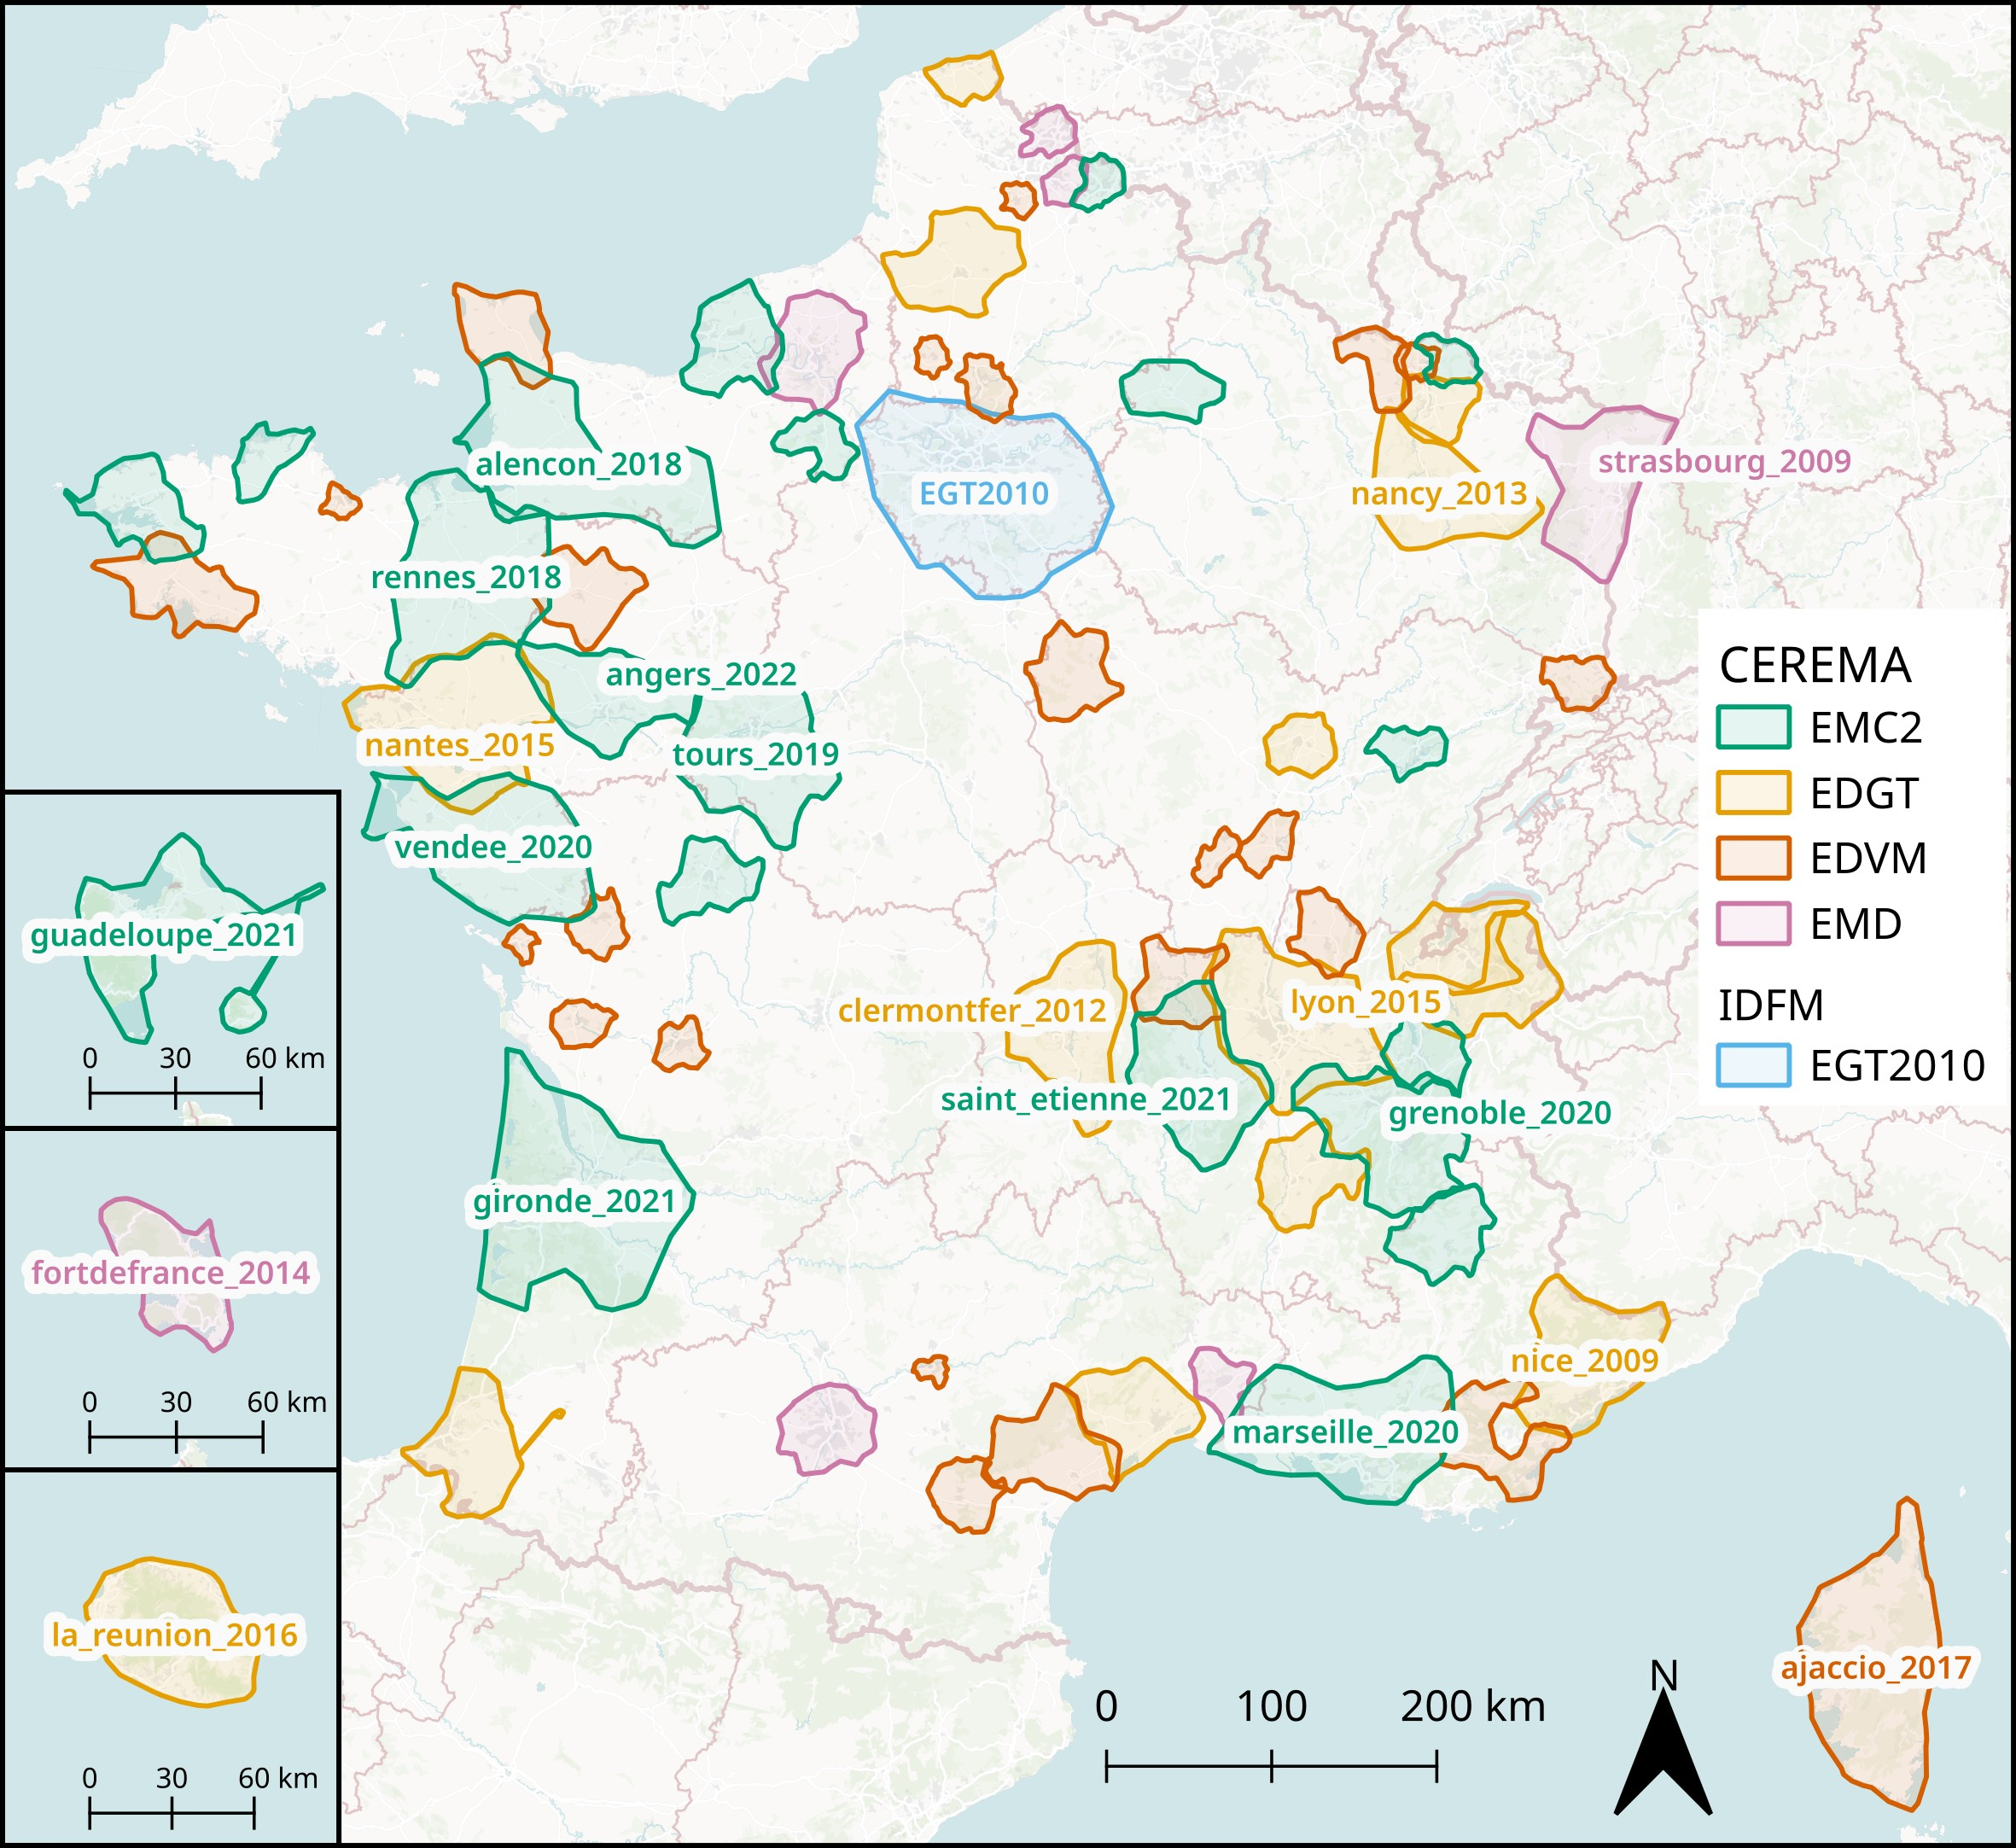
\includegraphics[height=0.8\textheight]{../../output/maps/survey_map.jpg}
        \end{column}
    \end{columns}
}

\frame{{\insertsection}{Couverture territoriale}
    \begin{columns}
        \begin{column}{.4\textwidth}
            \begin{itemize}
                \item Les 68 enquêtes couvrent environ \SI{62}{\%} de la France
                \item Les communes les moins densément peuplées sont les moins bien représentées
                \item Les ménages de communes à habitat rural très dispersé sont exclus (trop faible représentativité)
            \end{itemize}
        \end{column}
        \begin{column}{.6\textwidth}
            \centering
            \includegraphics{../../output/slides_graphs/insee_density_bars.pdf}
        \end{column}
    \end{columns}
}

\frame{{\insertsection}{(Re-)calage sur marge}
    \begin{columns}
        \begin{column}{.35\textwidth}
            Ajustement des pondérations d'origine des enquêtes pour répliquer les marges sur
            \begin{itemize}
                \item le genre (2 catégories)
                \item l'âge (8 catégories)
                \item la PCS (9 catégories)
                \item la densité de la commune (6 catégories)
            \end{itemize}
        \end{column}
        \begin{column}{.65\textwidth}
            \centering
            \includegraphics{../../output/slides_graphs/sample_weights_densities.pdf}
        \end{column}
    \end{columns}
}

\section{Analyse de l'intermodalité}

\frame{{\insertsection}{Outline}
    \tableofcontents[currentsection]
}

\frame{{\insertsection}{Rappels sur les enquêtes}
    \begin{itemize}
        \item \textbf{Déplacement :} mouvement d'une origine à une destination pour un motif donné (ex.~: travailler, s'éduquer, faire des achats)
        \item \textbf{Trajet :} segment continu utilisant un mode de transport unique
        \item Un déplacement est composé d'un ou de plusieurs trajets
    \end{itemize}
    \vspace{1em}
    \footnotesize
    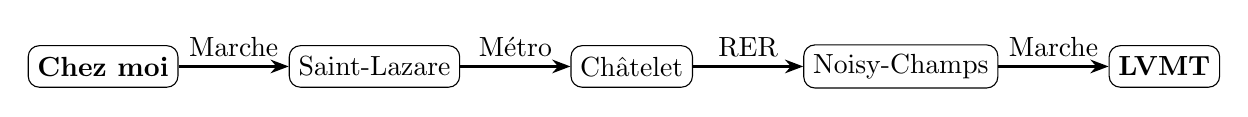
\begin{tikzpicture}[
        node distance=1.4cm,
        leg/.style={rectangle, draw, rounded corners, minimum height=1.5em, align=center},
        arrow/.style={-Stealth, thick}
        ]

        \node[leg] (home) {\textbf{Chez moi}};
        \node[leg, right=of home] (parking) {Saint-Lazare};
        \node[leg, right=of parking] (train_station) {Châtelet};
        \node[leg, right=of train_station] (work_station) {Noisy-Champs};
        \node[leg, right=of work_station] (work) {\textbf{LVMT}};

        \draw[arrow] (home) -- node[above] {Marche} (parking);
        \draw[arrow] (parking) -- node[above] {Métro} (train_station);
        \draw[arrow] (train_station) -- node[above] {RER} (work_station);
        \draw[arrow] (work_station) -- node[above] {Marche} (work);

    \end{tikzpicture}
}

\frame{{\insertsection}{Définition de l'intermodalité}
    Un \textbf{déplacement intermodal} est un déplacement contenant au moins deux trajets avec des modes différents
    \begin{itemize}
        \item Les trajets en marche à pied sont exclus de cette définition
        \item Les modes « transports en commun » (train, métro, bus, etc.) sont regroupés dans une même catégorie
        \item Modes considérés : voiture conducteur, voiture passager, transports en commun (TC), vélo, moto
    \end{itemize}
    \vspace{1em}
    \footnotesize
    
\begin{tikzpicture}[
        node distance=1.4cm,
        leg/.style={rectangle, draw, rounded corners, minimum height=1.5em, align=center},
        arrow/.style={-Stealth, thick}
        ]

        \node[leg] (home) {\textbf{Domicile}};
        \node[leg, right=of home] (parking) {Parking};
        \node[leg, right=of parking] (train_station) {Gare départ};
        \node[leg, right=of train_station] (work_station) {Gare arrivée};
        \node[leg, right=of work_station] (work) {\textbf{Travail}};

        \draw[arrow] (home) -- node[above] {Voiture} (parking);
        \draw[arrow] (parking) -- node[above] {Marche} (train_station);
        \draw[arrow] (train_station) -- node[above] {Train} (work_station);
        \draw[arrow] (work_station) -- node[above] {Marche} (work);

    \end{tikzpicture}

    \vspace{1em}
    \normalsize
    Note. Les déplacements non « locaux » (> \SI{80}{\kilo\meter}) sont exclus de l'analyse
}

\frame{{\insertsection}{Fait stylisé 1 : Une faible part des déplacements}
    Sur l'agrégation de 68 enquêtes mobilité :
    \begin{itemize}
        \item \num{17298} déplacements intermodaux (« poids » de 2.7 millions)
        \item \SI{1.2}{\%} des déplacements
        \item \SI{4.6}{\%} de la distance totale (à vol d'oiseau) parcourue
    \end{itemize}

    En Île-de-France (EGT 2010) :
    \begin{itemize}
        \item \SI{1.5}{\%} des déplacements
        \item \SI{7.1}{\%} de la distance totale (à vol d'oiseau) parcourue
    \end{itemize}
}

\frame{{\insertsection}{Fait stylisé 2 : Des déplacements longs}
    Distance moyenne :
    \begin{itemize}
        \item Déplacements intermodaux : \SI{20.7}{\kilo\meter}
        \item Déplacements unimodaux (hors MàP) : \SI{7.0}{\kilo\meter}
    \end{itemize}
    \centering
    \includegraphics{../../output/slides_graphs/euclidean_dist_densities.pdf}
}

\frame{{\insertsection}{Fait stylisé 3 : Déplacements pour un motif de travail ou d'éducation}
    \begin{columns}
        \begin{column}{.43\textwidth}
            Hiérarchie des déplacements de Raux et al.\ (2018)

            Part des motifs travail et éducation~:
            \begin{itemize}
                \item Déplacements intermodaux~: \SI{79}{\%}
                \item Déplacements unimodaux (hors MàP)~: \SI{43}{\%}
            \end{itemize}
        \end{column}
        \begin{column}{.57\textwidth}
            \centering
            \includegraphics{../../output/slides_graphs/purposes_bars.pdf}
        \end{column}
    \end{columns}
}

\frame{{\insertsection}{Fait stylisé 4 : Une majorité de combinaisons voiture + transports en commun}
    \begin{columns}
        \begin{column}{.4\textwidth}
            La combinaison de la voiture (conducteur ou passager) et des transports en commun représente \SI{85}{\%} des déplacements intermodaux
        \end{column}
        \begin{column}{.6\textwidth}
            \centering
            \includegraphics{../../output/slides_graphs/intermodality_types_bars.pdf}
        \end{column}
    \end{columns}
}

\frame{{\insertsection}{Fait stylisé 5 : La majorité de la distance est parcourue en transports en commun}
    Sur les déplacements voiture + TC, distance à vol d'oiseau moyenne :
    \begin{itemize}
        \item En transports en commun~: \SI{18.6}{\kilo\meter}
        \item En voiture~: \SI{5.2}{\kilo\meter}
    \end{itemize}
    \centering
    \includegraphics{../../output/slides_graphs/pt_dist_ratio_density.pdf}
}

\frame{{\insertsection}{Fait stylisé 6 : Le train et l'autocar comme modes principaux de correspondance}
    \begin{columns}
        \begin{column}{.47\textwidth}
            Usage du train :
            \begin{itemize}
                \item Correspondance Voiture $\leftrightarrow$ TC : \SI{44}{\%}
                \item Global : \SI{17}{\%}
            \end{itemize}
            Usage de l'autocar :
            \begin{itemize}
                \item Correspondance Voiture $\leftrightarrow$ TC : \SI{21}{\%}
                \item Global : \SI{11}{\%}
            \end{itemize}
        \end{column}
        \begin{column}{.53\textwidth}
            \centering
            \includegraphics{../../output/slides_graphs/pt_modes_bars.pdf}
        \end{column}
    \end{columns}
    \vspace{1em}
    Dans \SI{62}{\%} des cas, la partie TC ne comporte qu'un seul tronçon.
}

\frame{{\insertsection}{Fait stylisé 7 : Surreprésentation des étudiants et des personnes sans permis parmi les passagers de voiture}
    Voiture passager + Transports en commun :
    \begin{itemize}
        \item \SI{77}{\%} d'étudiants ou de personnes sans permis (vs \SI{22}{\%} au global)
    \end{itemize}

    Voiture conducteur + Transports en commun :
    \begin{itemize}
        \item Surreprésentation des cadres (\SI{31}{\%} vs \SI{19}{\%}) et des professions intermédiaires (\SI{34}{\%} vs \SI{25}{\%})
        \item Sous-représentation des ouvriers (\SI{7}{\%} vs \SI{18}{\%}) et des artisans (\SI{3}{\%} vs \SI{7}{\%})
    \end{itemize}
}

\frame{{\insertsection}{Fait stylisé 8 : Une connexion des milieux peu denses / ruraux vers les centres urbains}
    \begin{columns}
        \begin{column}{.55\textwidth}
            Grille de densité de l'INSEE en 3 niveaux (commune densément peuplée, de densité intermédiaire ou rurale) + distinction commune pôle de l'aire d'attraction (AAV)

            Parmi les déplacements Voiture$\rightarrow$TC :
            \begin{itemize}
                \item \SI{38}{\%} partent de communes rurales (vs \SI{26}{\%} pour les déplacements unimodaux)
                \item \SI{55}{\%} arrivent dans des communes pôle d'AAV (vs \SI{18}{\%} pour les déplacements unimodaux)
            \end{itemize}
        \end{column}
        \begin{column}{.45\textwidth}
            \centering
            \includegraphics{../../output/slides_graphs/insee_density_flows_polar.pdf}
        \end{column}
    \end{columns}
}

\frame{{\insertsection}{Bonus : Étude du choix de la gare de correspondance}
    \begin{columns}
        \begin{column}{.5\textwidth}
            \begin{itemize}
                \item Les enquêtes permettent de connaître l'origine et le lieu de correspondance à l'échelle de \emph{zones fines} (aire de \SI{6}{\kilo\meter\squared} en moyenne)
                \item La localisation des arrêts de transports en commun sur toute la France sont connues grâce aux fichiers GTFS
            \end{itemize}
        \end{column}
        \begin{column}{.5\textwidth}
            \centering
            \includegraphics[width=\textwidth]{../../output/maps/nearest_stop_zones_slides.jpg}
        \end{column}
    \end{columns}
}

\frame{{\insertsection}{Bonus : Étude du choix de la gare de correspondance}
    \begin{columns}
        \begin{column}{.5\textwidth}
            \begin{itemize}
                \item La gare utilisée est la plus proche si, pour tous les sommets de la \textbf{\textcolor{myblue}{zone d'origine}}, la gare la plus proche se situe dans la \textbf{\textcolor{myorange}{zone d'entrée}}
                \item La gare utilisée n'est \emph{pas} la plus proche si, pour tous les sommets de la \textbf{\textcolor{myblue}{zone d'origine}}, la gare la plus proche ne se situe \emph{pas} dans la \textbf{\textcolor{myorange}{zone d'entrée}}
                \item Dans les autres cas, on ne peut pas conclure
            \end{itemize}
        \end{column}
        \begin{column}{.5\textwidth}
            \centering
            \includegraphics[width=\textwidth]{../../output/maps/nearest_stop_example_slides.jpg}
        \end{column}
    \end{columns}
}

\frame{{\insertsection}{Bonus : Étude du choix de la gare de correspondance}
    \begin{itemize}
        \item Les utilisateurs du train prennent assez souvent la gare la plus proche (entre \SI{36}{\%} et \SI{66}{\%} des cas)
        \item Les utilisateurs du tramway et du métro semblent répondre à une autre logique (stationnement, ligne desservie, temps de trajet global)
    \end{itemize}
    \vspace{1em}
    \centering
    \begin{tabular}{lccc}
        \toprule
         & Train & Tramway & Métro \\
         \midrule
        Utilise l'arrêt le plus proche & \SI{36}{\%} & \SI{8}{\%} & \SI{19}{\%} \\
        N'utilise pas l'arrêt le plus proche & \SI{34}{\%} & \SI{69}{\%} & \SI{59}{\%} \\
        On ne sait pas & \SI{30}{\%} & \SI{23}{\%} & \SI{22}{\%} \\
        \bottomrule
    \end{tabular}
}

\frame[plain]{
    \centering
    {\Large\color{ColorOne}{\textbf{Merci pour votre attention}}}

    \vspace{2em}
    \flushleft
    Liens utiles :
    \begin{itemize}
        \item Standardisation des enquêtes avec MobiSurvStd : \url{https://mobisurvstd.github.io/MobiSurvStd}
        \item Code source pour reproduire les résultats : \url{https://github.com/LucasJavaudin/intermodality-analysis}
    \end{itemize}
}


\end{document}
